\documentclass[11pt,xcolor=svgnames]{beamer}

\usepackage[T1]{fontenc}
\usepackage[spanish]{babel}
\usepackage[utf8]{inputenc}

\usepackage{graphicx}
\usepackage{tikz}

\usepackage{charter}
\usepackage{inconsolata}
\usepackage{helvet}

\usetikzlibrary{arrows,shapes,snakes}

\usepackage{colores}

\usetheme{umbc2}
% \usefonttheme{serif}
\usefonttheme{structurebold}
\usecolortheme[named=Gray]{structure}

\title{oFlute: reconocimiento de señales aplicado al aprendizaje de la flauta
  dulce} 

\author{José Tomás Tocino García}

\institute[Universidad de Cádiz]{Universidad de Cádiz}

\date[Sept 2011]{Septiembre de 2011}

\AtBeginSection[]
{
  \begin{frame}<beamer>
    \frametitle{Índice}
   \transboxin
    \tableofcontents[currentsection,currentsubsection]
  \end{frame}

}

\defbeamertemplate*{title page}{customized}[1][]
{
  \vbox{}
  \vfill
  \begin{centering}
    \vspace{0.05cm}
    
\includegraphics[width=0.215\textwidth]{imagenes/logotipo} 
    \vspace{0.2cm}
    \begin{beamercolorbox}[sep=8pt,center,#1]{title}
      \usebeamerfont{title}\inserttitle\par%
    \end{beamercolorbox}%
    \vskip0.5em\par
    \begin{beamercolorbox}[sep=0pt,center,#1]{author}
      \usebeamerfont{author}\small\insertauthor\\
      \texttt{<josetomas.tocino@uca.es>}
    \end{beamercolorbox}
    \vspace{0.2cm}
    \begin{beamercolorbox}[sep=0pt,center,#1]{date}
      \usebeamerfont{date}
      {\scriptsize \insertdate }
    \end{beamercolorbox}%\vskip0.5em

    
\includegraphics[width=0.12\textwidth]{imagenes/logo_uca} 

    % {\usebeamercolor[fg]{titlegraphic}\inserttitlegraphic\par}
  \end{centering}
  \vfill

}

\setbeamercolor{footline}{fg=white, bg=white}

\begin{document}

% Transparencia de Inicio -> Título
{
  \setbeamertemplate{footline}{}
  \begin{frame}
    \titlepage
  \end{frame}
}
% \logo{
\includegraphics[height=2.5cm]{imagenes/logotipo}}
\setbeamertemplate{background}{
\includegraphics[width=\paperwidth,height=\paperheight]{imagenes/fondo1.pdf}}
\normalsize

% Transparencia de índice

\begin{frame}{Índice}
  \tableofcontents
\end{frame}


\section{Introducción}
\section{Contexto y motivación}
Las nuevas tecnologías van filtrándose gradualmente en los centros
educativos, y las técnicas de enseñanza se están adaptando a las
opciones que ofrecen. El reparto de ordenadores portátiles a los
alumnos andaluces de 5º y 6º de primaria, dentro del marco de la
Escuela TIC 2.0, es buena muestra de ello. 

Por otro lado, las nuevas generaciones están en plena simbiosis con
las tecnologías de la información, cada vez más acostumbradas al
empleo de dispositivos electrónicos, y su uso ya les es prácticamente
instintivo. Por tanto, es beneficioso buscar nuevos métodos educativos
que hagan uso de las nuevas tecnologías.

En la búsqueda de materias educativas en las que aplicar el uso de las
nuevas tecnologías, la música, parte fundamental del programa
curricular en la educación primaria, ofrece una gran variedad de
aspectos que podrían desarrollarse utilizando tecnologías de la
información. Es ahí donde este proyecto hace su aportación.

\section{Objetivos}
A la hora de definir los objetivos de un sistema, podemos agruparlos
en dos tipos diferentes: \textbf{funcionales} y
\textbf{transversales}. Los primeros se refieren a \textit{qué} debe
hacer la aplicación que vamos a desarrollar, e inciden
directamente en la experiencia del usuario y de potenciales
desarrolladores.

Por otro lado, los objetivos transversales son aquellos invisibles al
usuario final, pero que de forma inherente actúan sobre el resultado
final de la aplicación y sobre la experiencia de desarrollo de la misma.

\subsection{Funcionales}
\begin{itemize}
\item Crear un módulo de análisis del sonido en el dominio de la
  frecuencia para poder identificar las notas capturadas por el
  micrófono en tiempo real.
\item Crear una aplicación de usuario que identifique y muestre en
  pantalla las notas que toca el usuario en cada momento.
\item Reutilizar el módulo de análisis en un juego en el que el
  usuario debe tocar correctamente las notas que aparecen en pantalla
  siguiendo un pentagrama.
\item Incluir un sistema de lecciones multimedia individuales que
  sirvan al alumno de referencia y fuente de aprendizaje.
\item Potenciar el uso de interfaces de usuario amigables, con un
  sistema avanzado de animaciones que proporcione un aspecto fluido y
  evite saltos bruscos entre secciones.
\end{itemize}

\subsection{Transversales}
\begin{itemize}
\item Obtener una base teórica sobre cómo se representa y caracteriza
  digitalmente el sonido.
\item Conocer las bases del \ac{DSP}, y su uso en aplicaciones de
  reconocimiento básico de sonidos, tales como sintonizadores y
  afinadores de instrumentos.
\item Introducirme en la programación de audio en sistemas GNU/Linux.
\item Entender las bases del análisis de sonidos en el dominio de la
  frecuencia. 
\item Utilizar un enfoque de análisis, diseño y codificación orientado
  a objetos, de una forma lo más clara y modular posible, para
  permitir ampliaciones y modificaciones sobre la aplicación por
  terceras personas.
\item Hacer uso de herramientas básicas en el desarrollo de software,
  como son los \textbf{Sistemas de Control de Versiones} para llevar
  un control realista del desarrollo del software, así como hacer de
  las veces de sistema de copias de seguridad.
\end{itemize}


\section{Alcance}
\textbf{oFlute} se modela como una herramienta lúdico-educativa para
alumnos que comiencen a aprender a usar la flauta dulce,
proporcionando un entorno atractivo y ameno para el estudiante. Éstos
tendrán la posibilidad de recorrer una serie de pequeñas lecciones
sobre música en general, y el uso de la flauta dulce en particular.

Además, el usuario tendrá la posibilidad de comprobar sus
conocimientos sobre el uso de la flauta practicando, gracias a las
secciones de análisis de notas y de canciones, en las que la
aplicación valorará la pericia del estudiante con la flauta.  

\subsection{Limitaciones del proyecto}
El proyecto se limita al uso de la flauta dulce y no a otros
instrumentos por la enorme variabilidad de timbre entre ellos, lo que
supondría un enorme esfuerzo a la hora de generalizar el analizador de
frecuencias.

El sistema de lecciones se basa en plantillas XML en las que es
posible definir imágenes y texto para formar una pantalla
de información. En un futuro se ampliará para incluir otros elementos
multimedia así como lecciones con varias pantallas consecutivas.

Los sistemas de audio son una de las áreas en las que menos consenso hay entre
plataformas informáticas, por lo que la transportabilidad de las aplicaciones
suele ser compleja. El presente proyecto utiliza la API Simple de PulseAudio
como subsistema de sonido, que es en teoría compatible con plataformas Win32,
pero en la práctica su complejidad hace prácticamente inviable la portabilidad
de la aplicación.

\subsection{Licencia}
El proyecto está publicado como software libre bajo la licencia
\ac{GPL} versión 2. El conjunto de bibliotecas y módulos utilizados
tienen las siguientes licencias:
\begin{itemize}

\item A lo largo del proyecto se utilizan diferentes partes de las
  bibliotecas \textbf{Boost}~\cite{boost}, que utilizan la licencia
  \textit{Boost Software License}~\footnote{\url{http://www.boost.org/LICENSE_1_0.txt}}.
  Se trata de una licencia de software libre, compatible con la GPL, y
  comparable en permisividad a las licencias BSD y MIT.

\item \textbf{Gosu}~\cite{gosu}, la biblioteca de desarrollo de
  videojuegos que ha proporcionado el subsistema gráfico, utiliza la
  licencia \ac{MIT}. Cuando se compila en sistemas Windows, utiliza la
  biblioteca FMOD que es gratuita pero de código cerrado; en sistemas
  GNU/Linux, utiliza SDL\_mixer, que utiliza la licencia \ac{LGPL}.

\item \textbf{Kiss FFT}~\cite{kissfft}, la biblioteca utilizada para
  hacer el análisis de frecuencias, utiliza una licencia \ac{BSD}.

\item \textbf{PugiXML}~\cite{pugixml}, biblioteca de procesamiento de
  ficheros XML, se distribuye bajo al licencia MIT.

\item \textbf{PulseAudio}~\cite{pulseaudio} utiliza una licencia LGPL 2.1.
\end{itemize}

\section{Estructura del documento}
El presente documento se rige según la siguiente estructura:

\begin{itemize}
\item \textbf{Introducción}. Se exponen las motivaciones y objetivos detrás del
  proyecto \textbf{oFlute}, así como información sobre las licencias de sus
  componentes, glosario y estructura del documento.
\item \textbf{Desarrollo del calendario}, donde se explica la planificación del
  proyecto, la división de sus etapas, la extensión de las etapas a lo largo del
  tiempo y los porcentajes de esfuerzo.
\item \textbf{Investigación preliminar}, que explica las labores de
  documentación y experimentación previas al desarrollo, que han servido para
  labrar una base de conocimientos que nos diera las suficientes garantías para
  afrontar el proyecto.
\item \textbf{Análisis}. Se detalla la fase de análisis del sistema, explicando
  los requisitos funcionales del sistema, los diferentes casos de uso, así como
  las principales operaciones con sus diagramas de secuencia y contratos.
\item \textbf{Diseño}. Seguido del análisis, se expone en detalle la etapa de
  diseño del sistema, con los diagramas de clases.
\item \textbf{Implementación}. Una vez analizado el sistema y definido su
  diseño, en esta parte se detallan las decisiones de implementación más
  relevantes que tuvieron lugar durante el desarrollo del proyecto.
\item \textbf{Pruebas}. Listamos y describimos las pruebas que se han llevado a
  cabo sobre el proyecto para garantizar su fiabilidad y consistencia.
\marginpar{RELLENAR}
\end{itemize}

Tras una revisión del calendario seguido, detallaremos a lo largo del
resto de la memoria el proceso de análisis, diseño, codificación y
pruebas que se siguió al realizar el proyecto.  

Los manuales de usuario y de instalación se incluyen tras un resumen
de los aspectos más destacables de proyecto y las conclusiones. En
dicho manual, se hallan dos apartados dirigidos a la ampliación de la
aplicación mediante la creación de nuevas lecciones y de nuevas
canciones, respectivamente.



\section{Descripción}

\section{Perspectiva del producto}

\section{Funciones}

Lista de funciones

\section{Características de los usuarios}

\section{Restricciones generales}

\section{Suposiciones y dependencias}


\section{Requisitos para futuras versiones}









\section{Calendario}
El proyecto no se ha desarrollado siguiendo un calendario estricto,
dado que era imposible cuantificar el tiempo que tomaría el adquirir
las bases teóricas necesarias para poder afrontarlo con garantías. Su
desarrollo se ha compaginado con los estudios del último curso de
Ingeniería Técnica en Informática de Sistemas y las labores como
becario en la Oficina de Software Libre y Conocimiento Abierto de la
Universidad de Cádiz~\cite{osluca}.

\section{Iteraciones}

Para la realización del presente proyecto se ha utilizado un modelo de
desarrollo iterativo incremental. A continuación se detallan cada una
de las etapas por las que ha ido pasando el software, y se observará
como conforme se iba avanzando se añadían nuevas funcionalidades y se
pulían las existentes.

\section{Diagrama de Gantt}

\section{Porcentajes de esfuerzo}



\section{Fundamentos teóricos}
\begin{frame}{El sonido}
  \begin{center}
    El \textbf{sonido} es una vibración en forma de onda.

    \bigskip
    \bigskip

    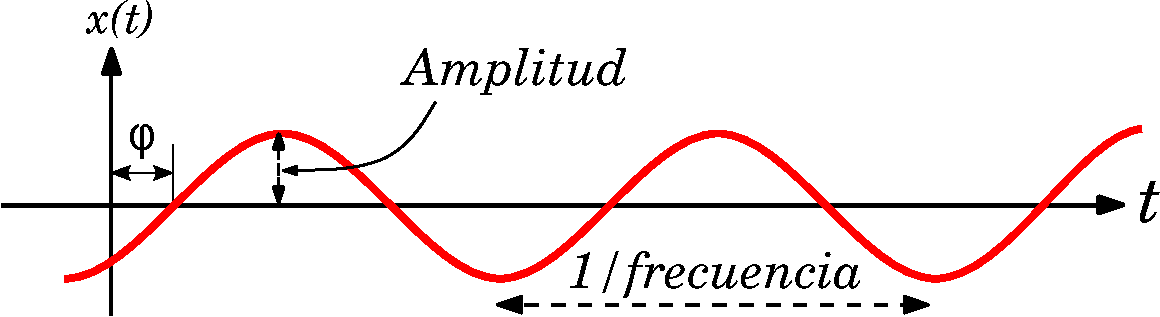
\includegraphics[width=0.8\textwidth]{imagenes/imagen_onda}

    \bigskip

    \begin{description}
    \item[Frecuencia] Oscilaciones por unidad de tiempo. 
    \item[Amplitud] Energía que transporta la onda.
    \item[Fase] Desplazamiento respecto del origen.
    \end{description}
  \end{center}
\end{frame}

\begin{frame}{Descomposición de sonidos}
  \begin{center}
    Los sonidos no suelen ser ondas puras, \\se componen de \textbf{parciales}.

    \pause \bigskip
  
    La \textbf{frecuencia fundamental} es el menor de esos parciales. Dicta la
    \textbf{altura} general del sonido, esto es, la \textbf{nota}.

    \pause \bigskip

    Los \textbf{armónicos} son parciales múltiplos de la frecuencia fundamental,
    enriquecen y caracterizan el sonido. 

    \pause \bigskip
  
    {\large
    \textcolor{red}{\textbf{Objetivo:}} Descomponer el sonido para obtener la \\
    \textbf{frecuencia fundamental}.}
  \end{center}
\end{frame}

\begin{frame}{Herramientas de análisis armónico}
  \begin{center}
    Trabajan en el \textbf{dominio de la frecuencia}: se representa una señal
    respecto a su espectro de frecuencias.

    \pause \bigskip

    La \textbf{transformada de Fourier} es la herramienta más conocida:
    descompone una señal en sus componentes senoidales.

    \pause \bigskip

    Algoritmo más habitual: \textbf{FFT - Fast Fourier Transform}. \\En nuestro
    caso usamos la versión discreta, \\\textbf{DFT - Discrete Fourier Transform}.

  \end{center}
\end{frame}

\begin{frame}{Ejemplo de aplicación de FFT}
  \begin{center}
    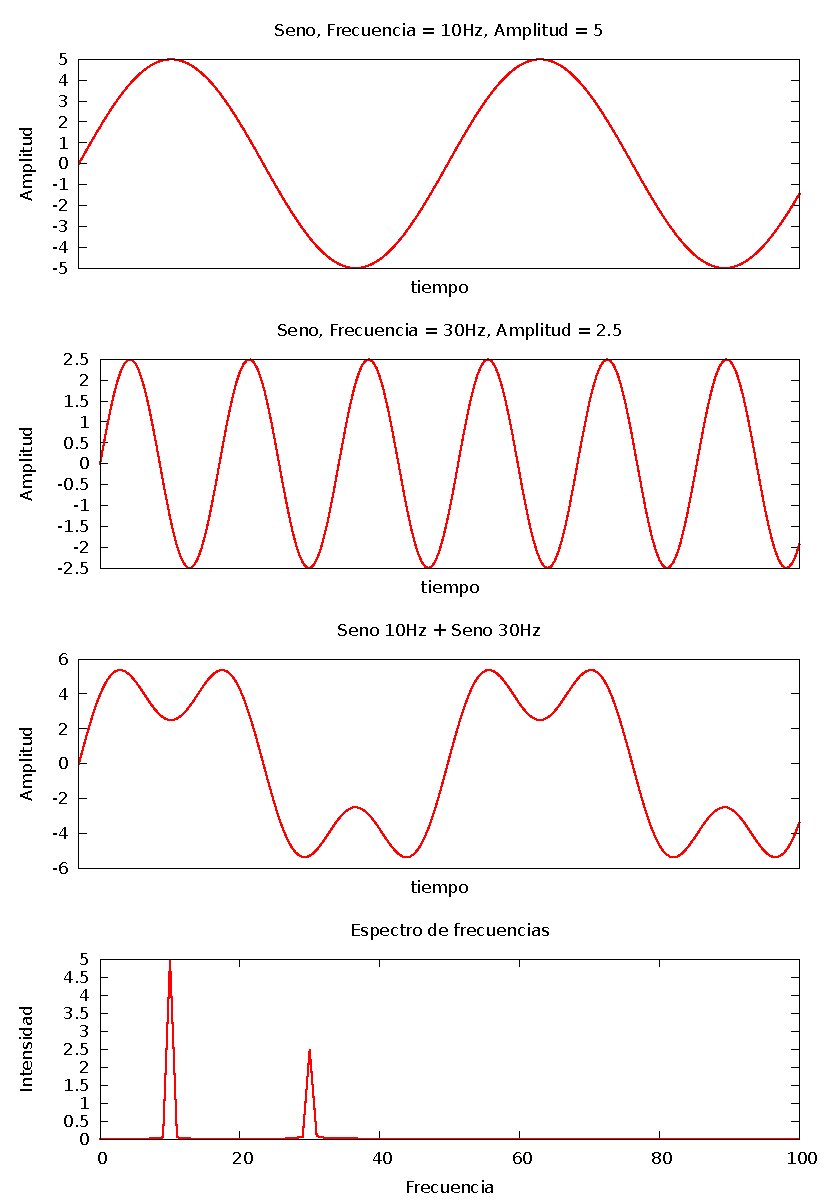
\includegraphics[width=\textwidth]{scripts_octave/imagen_senosEspectro}
  \end{center}
\end{frame}

\begin{frame}{Función ventana}
  \begin{center}
    Se aplica sobre el conjunto de entrada, suaviza la señal.

    \medskip

    Hay muchos tipos, según la respuesta de salida: Hann, Hamming, gausiana, Tukey, Lanczos...

    \medskip

    Ejemplo de ventana de Hann:

    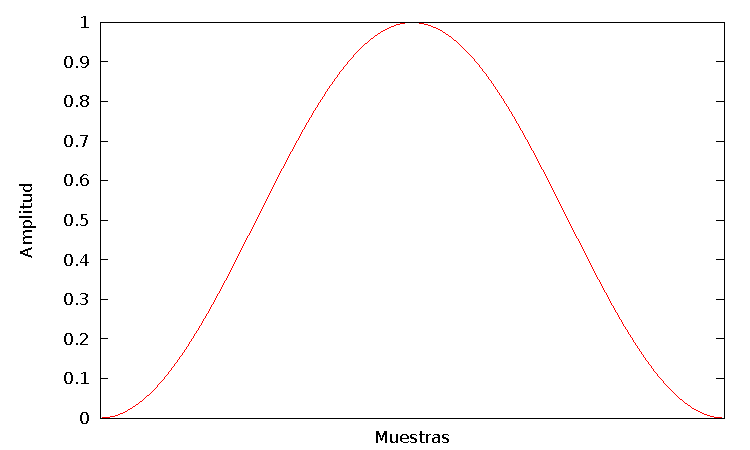
\includegraphics[width=0.5\textwidth]{scripts_octave/imagen_hann}

    \medskip

    En oFlute no se utiliza.
  \end{center}
\end{frame}

%%% Local Variables: 
%%% mode: latex
%%% TeX-master: "../presentacion"
%%% End: 


\section{Desarrollo}
\begin{frame}{Analizador básico}
  \begin{block}{Objetivo}
    Desarrollar un módulo que capture el sonido del micrófono, lo analice y
    detecte la nota que se está tocando.
  \end{block}

  \pause

  \begin{block}{Primer paso: capturar el audio}
    \begin{itemize}
    \item Se utilizó la API de PulseAudio.
    \item Abrimos un flujo de entrada.
    \item Creamos un búffer para recoger los datos.
    \item Procesamos los datos cuando se llena el búffer.
    \end{itemize}
    
  \end{block}
\end{frame}

\begin{frame}{Analizador básico}
  \begin{block}{Segundo paso: analizar el sonido}
    \begin{itemize}
    \item Trabajamos con el contenido del búffer.
    \item Aplicamos el algoritmo DFT.
    \item Aislamos la frecuencia fundamental.
    \item Comparamos la frecuencia fundamental con una tabla de frecuencias para
      la flauta dulce.
    \item Devolvemos la nota detectada.
    \end{itemize}
  \end{block}  
\end{frame}

\begin{frame}[fragile]{Carga de fuentes TrueType}
  \begin{center}
    oFlute utiliza \textbf{Gosu} como sistema gráfico.
    
    \pause
    \medskip
    
    \textcolor{red}{\textbf{Problema:}} Gosu no permite cargar fuentes TrueType
    en GNU/Linux.

    \pause
    \medskip
    
    \textcolor{dgreen}{\textbf{Solución:}} se implementa un módulo propio para
    carga y pintado de fuentes TrueType. \pause\\[1em]Este módulo se liberó y pasó a
    formar \textbf{parte oficial} de Gosu.
  \end{center}
  \begin{minted}{cpp}
// Used for custom TTF files
// Adapted from customFont class by Jose Tomas Tocino Garcia (TheOm3ga)
class SDLTTFRenderer : boost::noncopyable
  \end{minted}
\end{frame}

\begin{frame}{Animaciones dinámicas}
  \begin{center}
    \textcolor{red}{\textbf{Problema:}} uno de los objetivos era tener
    interfaces amigables, fluidas y minimalistas.

    \pause \medskip

    \textcolor{dgreen}{\textbf{Solución:}} se desarrolla un sistema de
    animaciones mediante interpolaciones de movimiento.

    \pause\medskip

    Permite movimientos de aceleración, deceleración, uniformes, etcétera. Es
    extensible a un número arbitrario de atributos.

    \pause\medskip

    Se basó en las ecuaciones de Robert Penner, \\liberadas bajo licencia BSD.
    
  \end{center}  
\end{frame}

%%% Local Variables: 
%%% mode: latex
%%% TeX-master: "../presentacion"
%%% End: 


\section{Herramientas}


\section{Conclusiones y difusión}

\section{Bibliografía}
{
  \setbeamertemplate{background}{
\includegraphics[width=\paperwidth,height=\paperheight]{imagenes/fondo_simple.pdf}}
  \begin{frame}
    \frametitle{}
    
    \begin{center}

      
\includegraphics[scale=1]{imagenes/logotipo}
      
      \bigskip
      \bigskip

      {\Large Demostración}

    \end{center}

  \end{frame}

  \begin{frame}{}
    
    \begin{center}
      
\includegraphics[scale=0.8]{imagenes/logotipo}

      \bigskip
      \bigskip

      {\LARGE Gracias por su atención}\\

      \medskip

      {\large ¿Preguntas?}\\

      \bigskip
      \medskip

      {\large \url{http://oflute.googlecode.com} \\[0.3em] \url{http://oflute.wordpress.com}}
    \end{center}

  \end{frame}
}


%%% Local Variables: 
%%% mode: latex
%%% TeX-master: "../presentacion"
%%% End: 


\end{document}

%%% Local Variables: 
%%% mode: latex
%%% TeX-master: t
%%% End: 
